%% GENERATED by tools/from_docs.py from stepss-docs. Do not edit by hand:
%% edit the page named below in stepss-docs and regenerate.
%% source: stepss-docs/src/content/docs/models/governors/generic.mdx

\chapter{Basic and generic turbine-governor models}\label{doc:model-tor-generic}

This page documents the four governors built into every RAMSES distribution, \texttt{CONSTANT}, \texttt{1ST\_ORDER}, \texttt{HYDRO\_GENERIC1} and \texttt{THERMAL\_GENERIC1}, which take no prefix and are written in uppercase, together with \texttt{HYDRO\_DG}, registered since 3.76.

The \texttt{TOR} sub-record these models are entered with is described on the \hyperref[doc:model-tor]{Governor Models} page.

\section{\texorpdfstring{CONSTANT (\texttt{tor\_constant})}{CONSTANT (tor\_constant)}}\label{model-tor-generic:constant-tor_constant}

The data-file model name is \texttt{CONSTANT}.

\subsection{Scientific Description}\label{model-tor-generic:scientific-description}

The \texttt{tor\_constant} model provides a \textbf{constant mechanical torque} source. The mechanical torque is fixed at its initialisation value and does not respond to speed deviations or load changes:

\[T_m(t) = T_{m0} \quad \forall t\]

The single algebraic state satisfies:

\[f(1) = x(1) - T_{m0} = 0\]

The observable output is mechanical power:

\[P_m = T_m \cdot \omega\]

\textbf{Implementation details:}
- \texttt{nbxvar\ =\ 1}, \texttt{nbzvar\ =\ 0}, \texttt{nbdata\ =\ 0}
- One additional parameter: \texttt{prm(1)\ =\ Tm0} (set at initialisation from load-flow)
- Observable: \texttt{Pm\ =\ x(1)\ *\ omega}

\subsection{Parameters}\label{model-tor-generic:parameters}

\begin{small}\begin{longtable}[]{@{}
  >{\raggedright\arraybackslash}p{(\linewidth - 4\tabcolsep) * \real{0.2899}}
  >{\raggedright\arraybackslash}p{(\linewidth - 4\tabcolsep) * \real{0.7101}}
@{}}
\toprule\noalign{}
\begin{minipage}[b]{\linewidth}\raggedright
Parameter
\end{minipage} & \begin{minipage}[b]{\linewidth}\raggedright
Description
\end{minipage} \\
\midrule\noalign{}
\endhead
\bottomrule\noalign{}
\endlastfoot
\emph{(none)} & No user-supplied parameters. \(T_{m0}\) is taken from the load-flow initialisation. \\
\end{longtable}\end{small}

\subsection{Usage Example}\label{model-tor-generic:usage-example}

\textbf{RAMSES Data File}

\begin{Verbatim}
SYNC_MACH  g6  g6
      # FP FQ P Q: share of the power-flow injection (FP, FQ) or initial power (P in MW, Q in Mvar)
      1.  1.  0.  0.
      # SNOM: Nominal apparent power, used as base power in the machine model (MVA)
      400.
      # Pnom: Nominal active power of the turbine, used as base power for the turbine model (MW)
      360.
      # H: Inertia constant (s)
      6.
      # D: Damping coefficient (usually set to zero when the damper windings are modelled) (pu)
      0.
      # IBRATIO: Field current base ratio I_fB^mac/I_fB^exc (see above) (pu)
      2.05
      # TYPE_MOD: Parameter format keyword: RL or XT (case-insensitive)
      XT
      # Xl: Leakage reactance L_l (pu)
      0.15
      # Xd: d-axis synchronous reactance (pu)
      2.2
      # X'd: d-axis transient reactance (must be smaller than Xd) (pu)
      0.3
      # X"d: d-axis subtransient reactance (pu)
      0.2
      # Xq: q-axis synchronous reactance (pu)
      2.
      # X'q: q-axis transient reactance (pu)
      0.4
      # X"q: q-axis subtransient reactance (pu)
      0.2
      # m: Saturation coefficient (set to 0 to neglect saturation)
      0.1
      # n: Saturation exponent (ignored when m = 0)
      6.0257
      # Ra: Armature resistance (pu)
      0.
      # T'do: d-axis open-circuit transient time constant (s)
      7.00
      # T"do: d-axis open-circuit subtransient time constant (s)
      0.05
      # T'qo: q-axis open-circuit transient time constant (s)
      1.5
      # T"qo: q-axis open-circuit subtransient time constant (s)
      0.05
EXC  GENERIC1
      # IFLIM: OEL field current threshold (pu)
      3.0618
      # d: OEL timer band, usually negative: timer runs down at rate 1 below IFLIM+d, holds between IFLIM+d and IFLIM (pu)
      -0.1
      # f: OEL timer charging rate offset above IFLIM
      1.
      # S: OEL timer charging rate per unit of field overcurrent (1/pu)
      0.
      # K1: Not used by the code
      100.
      # K2: OEL gain on (if - IFLIM), negative so that the OEL lowers excitation (pu/pu)
      -1.
      # L1: OEL timer lower limit and initial value, negative; the OEL acts when the timer exceeds 0 (s)
      -20.0
      # L2: OEL timer upper limit (s)
      10.
      # G: AVR gain (pu/pu)
      120.
      # TA: AVR lead time constant (s)
      5.
      # TB: AVR lag time constant (s)
      12.5
      # TE: Exciter time constant (s)
      0.1
      # L3: Minimum field voltage (pu)
      0.
      # L4: Maximum field voltage (pu)
      5.
      # SPEEDIN: PSS input weight: 1 = speed, 0 = active power
      1
      # KPSS: PSS gain, derivative washout KPSS s/(1+sTw); 0 disables PSS (pu s)
      75.
      # Tw: PSS washout time constant (s)
      15.
      # T1: PSS first lead-lag numerator time constant (s)
      0.22
      # T2: PSS first lead-lag denominator time constant (s)
      0.012
      # T3: PSS second lead-lag numerator time constant (s)
      0.22
      # T4: PSS second lead-lag denominator time constant (s)
      0.012
      # DVMIN: PSS output lower limit (pu)
      -0.1
      # DVMAX: PSS output upper limit (pu)
      0.1
TOR  CONSTANT
;
\end{Verbatim}

\textbf{Notes}

\begin{itemize}
\tightlist
\item
  Useful for machines operating at fixed setpoint, for testing generator models in isolation, or as a placeholder.
\item
  The mechanical power observable \(P_m = T_m \cdot \omega\) will vary slightly with speed changes.
\item
  \texttt{TOR\ CONSTANT} takes no parameters, \(T_{m0}\) is set automatically from the load-flow initialisation.
\end{itemize}

\begin{center}\rule{0.5\linewidth}{0.5pt}\end{center}

\section{\texorpdfstring{1ST\_ORDER (\texttt{tor\_1storder})}{1ST\_ORDER (tor\_1storder)}}\label{model-tor-generic:st_order-tor_1storder}

The data-file model name is \texttt{1ST\_ORDER} (uppercase, with the underscore).

\subsection{Scientific Description}\label{model-tor-generic:scientific-description-1}

The \texttt{tor\_1storder} model is a \textbf{first-order speed governor} with droop and a two-mass (HP/LP) turbine representation. It captures the primary frequency response through a proportional-droop speed controller with a first-order lag.

\textbf{Speed controller with droop \(R\):}

The mechanical torque setpoint is:

\[T_{set} = T_{m0} - \frac{\omega - 1}{R}\]

The HP torque tracks \(T_{set}\) through a first-order lag with time constant \(T_2\):

\[\frac{d x_1}{dt} = \frac{1}{T_2}\left(T_{set} - x_1\right)\]

The LP (shaft) torque is a weighted combination:

\[x_2 = (1 - F_{HP}) \cdot x_1 + F_{HP} \cdot T_{set}\]

where \(F_{HP}\) is the fraction of power generated in the HP stage.

From the Fortran equations:

\begin{Verbatim}
f(1) = (-x(1) + (prm(4) - (omega-1.d0)/prm(3))) / prm(2)
f(2) = (1.d0-prm(1))*x(1) + prm(1)*(prm(4)-(omega-1.d0)/prm(3)) - x(2)
\end{Verbatim}

i.e.:
- \texttt{prm(1)\ =\ FHP} (HP fraction), \texttt{prm(2)\ =\ T2} (time constant), \texttt{prm(3)\ =\ R} (droop)
- \texttt{prm(4)\ =\ Tm0} (setpoint, set at init)

\textbf{Implementation details:}
- \texttt{nbxvar\ =\ 2}, \texttt{nbzvar\ =\ 0}, \texttt{nbdata\ =\ 3}
- State 1 = HP torque \texttt{x(1)}, State 2 = LP torque \texttt{x(2)}
- Observables: \texttt{HP\ torque}, \texttt{LP\ torque}

\begin{figure}[htbp]
\centering
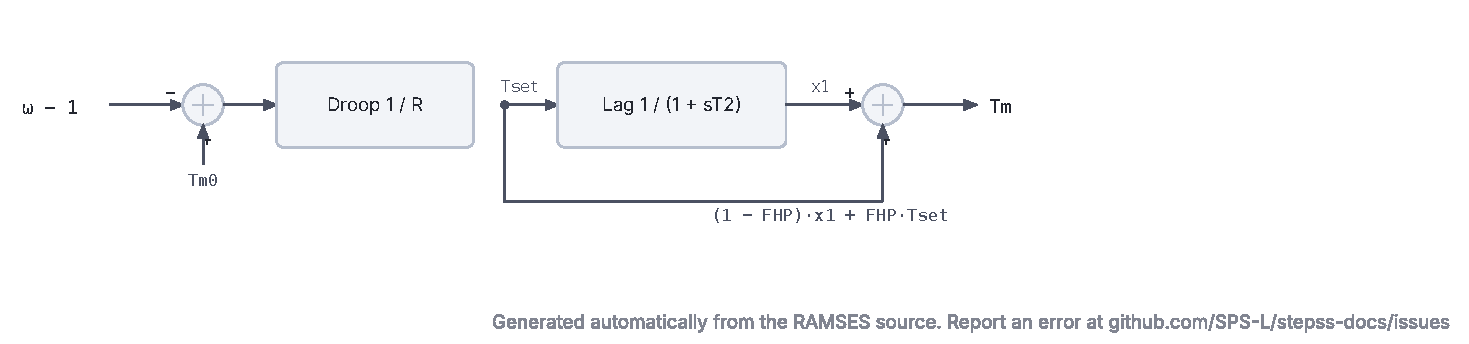
\includegraphics[width=0.98\linewidth]{figures/tor-1storder-light}
\caption{1ST\_ORDER governor block diagram.}
\end{figure}

\subsection{Parameters}\label{model-tor-generic:parameters-1}

\begin{small}\begin{longtable}[]{@{}ll@{}}
\toprule\noalign{}
Parameter & Description \\
\midrule\noalign{}
\endhead
\bottomrule\noalign{}
\endlastfoot
\texttt{FHP} & Fraction of torque produced by the HP turbine stage (0--1) \\
\texttt{T2} & Governor/HP turbine time constant (s) \\
\texttt{R} & Speed droop (pu/pu) \\
\end{longtable}\end{small}

\subsection{Usage Example}\label{model-tor-generic:usage-example-1}

\textbf{RAMSES Data File}

\begin{Verbatim}
SYNC_MACH  g1  g1
      # FP FQ P Q: share of the power-flow injection (FP, FQ) or initial power (P in MW, Q in Mvar)
      1.  1.  0.  0.
      # SNOM: Nominal apparent power, used as base power in the machine model (MVA)
      800.
      # Pnom: Nominal active power of the turbine, used as base power for the turbine model (MW)
      760.
      # H: Inertia constant (s)
      3.
      # D: Damping coefficient (usually set to zero when the damper windings are modelled) (pu)
      0.
      # IBRATIO: Field current base ratio I_fB^mac/I_fB^exc (see above) (pu)
      0.95
      # TYPE_MOD: Parameter format keyword: RL or XT (case-insensitive)
      XT
      # Xl: Leakage reactance L_l (pu)
      0.15
      # Xd: d-axis synchronous reactance (pu)
      1.1
      # X'd: d-axis transient reactance (must be smaller than Xd) (pu)
      0.25
      # X"d: d-axis subtransient reactance (pu)
      0.2
      # Xq: q-axis synchronous reactance (pu)
      0.7
      # X'q: q-axis transient reactance (pu)
      *
      # X"q: q-axis subtransient reactance (pu)
      0.2
      # m: Saturation coefficient (set to 0 to neglect saturation)
      0.1
      # n: Saturation exponent (ignored when m = 0)
      6.0257
      # Ra: Armature resistance (pu)
      0.
      # T'do: d-axis open-circuit transient time constant (s)
      5.00
      # T"do: d-axis open-circuit subtransient time constant (s)
      0.05
      # T'qo: q-axis open-circuit transient time constant (s)
      *
      # T"qo: q-axis open-circuit subtransient time constant (s)
      0.1
EXC  GENERIC1
      # IFLIM: OEL field current threshold (pu)
      1.8991
      # d: OEL timer band, usually negative: timer runs down at rate 1 below IFLIM+d, holds between IFLIM+d and IFLIM (pu)
      -0.1
      # f: OEL timer charging rate offset above IFLIM
      0.
      # S: OEL timer charging rate per unit of field overcurrent (1/pu)
      1.
      # K1: Not used by the code
      100.
      # K2: OEL gain on (if - IFLIM), negative so that the OEL lowers excitation (pu/pu)
      -1.
      # L1: OEL timer lower limit and initial value, negative; the OEL acts when the timer exceeds 0 (s)
      -11
      # L2: OEL timer upper limit (s)
      10.
      # G: AVR gain (pu/pu)
      70.
      # TA: AVR lead time constant (s)
      10.
      # TB: AVR lag time constant (s)
      20.
      # TE: Exciter time constant (s)
      0.1
      # L3: Minimum field voltage (pu)
      0.
      # L4: Maximum field voltage (pu)
      4.
      # SPEEDIN: PSS input weight: 1 = speed, 0 = active power
      1
      # KPSS: PSS gain, derivative washout KPSS s/(1+sTw); 0 disables PSS (pu s)
      75.
      # Tw: PSS washout time constant (s)
      15.
      # T1: PSS first lead-lag numerator time constant (s)
      0.2
      # T2: PSS first lead-lag denominator time constant (s)
      0.01
      # T3: PSS second lead-lag numerator time constant (s)
      0.2
      # T4: PSS second lead-lag denominator time constant (s)
      0.01
      # DVMIN: PSS output lower limit (pu)
      -0.1
      # DVMAX: PSS output upper limit (pu)
      0.1
TOR  1ST_ORDER
      # FHP: fraction of torque following the setpoint without lag (HP part)
      0.30
      # T2: time constant of the lagged (LP) torque part (s)
      0.50
      # R: speed droop (pu)
      0.05
;
\end{Verbatim}

\textbf{Notes}

\begin{itemize}
\tightlist
\item
  \texttt{FHP\ =\ 0} makes the model a pure first-order lag on the total torque.
\item
  \texttt{FHP\ =\ 1} bypasses the HP lag entirely; the torque instantly tracks the droop setpoint.
\item
  Typical primary-frequency response studies use \texttt{R\ =\ 0.04}--\texttt{0.05}.
\end{itemize}

\begin{center}\rule{0.5\linewidth}{0.5pt}\end{center}

\section{\texorpdfstring{THERMAL\_GENERIC1 (\texttt{tor\_thermal\_generic1})}{THERMAL\_GENERIC1 (tor\_thermal\_generic1)}}\label{model-tor-generic:thermal_generic1-tor_thermal_generic1}

The data-file model name is \texttt{THERMAL\_GENERIC1}.

\subsection{Scientific Description}\label{model-tor-generic:scientific-description-2}

The \texttt{tor\_thermal\_generic1} model is a \textbf{generic multi-stage steam turbine governor}, suitable for both single-shaft and cross-compound units. It includes a speed controller with rate-limiting, a three-section steam chest/reheater, and separate HP, MP, and LP turbine stages.

\begin{figure}[htbp]
\centering
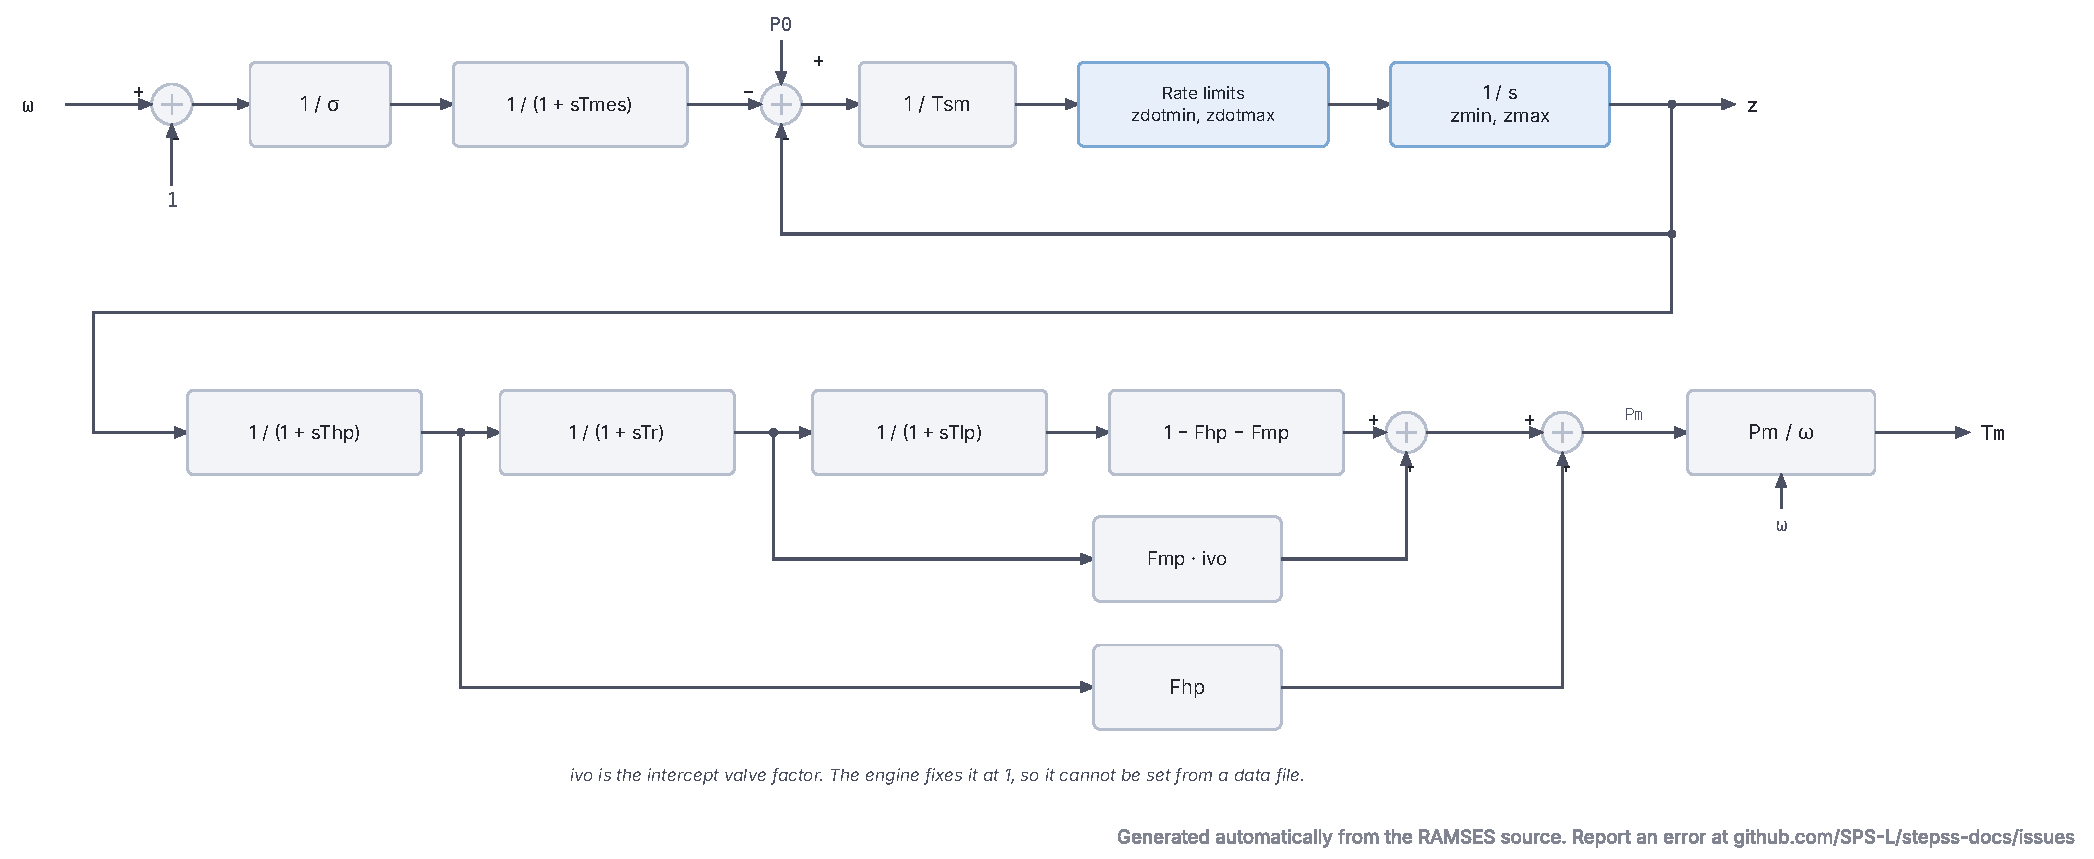
\includegraphics[width=0.98\linewidth]{figures/tor-thermal-generic1-light}
\caption{THERMAL\_GENERIC1 block diagram.}
\end{figure}

\textbf{Speed governor:}

The speed deviation is divided by the droop \(\sigma\) and measured with time constant \(T_{mes}\):

\[T_{mes}\,\dot{x}_1 = -x_1 + \frac{\omega - 1}{\sigma}\]

The gate demand is what remains of the power setpoint after that term and the current gate position are taken off:

\[e_{gov} = P_0 - x_1 - z\]

It is divided by the servo time constant \(T_{sm}\), rate-limited to \([zdot_{min},\, zdot_{max}]\), and integrated into the gate opening \(z\) within \([z_{min},\, z_{max}]\).

\textbf{Turbine power stages:}

The gate opening drives three lags in series, the reheat stage carrying the intercept valve factor \(ivo\):

\[T_{hp}\,\dot{x}_{hp} = -x_{hp} + z, \qquad
T_r\,\dot{x}_r = -x_r + x_{hp}, \qquad
T_{lp}\,\dot{x}_{lp} = -x_{lp} + ivo\,x_r\]

Each stage contributes its own fraction of the power, and the three fractions sum to one:

\[P_{mHP} = F_{hp}\,x_{hp}, \qquad
P_{mMP} = F_{mp}\,ivo\,x_r, \qquad
P_{mLP} = (1 - F_{hp} - F_{mp})\,x_{lp}\]

Total mechanical power, and the torque delivered to the shaft:

\[P_m = P_{mHP} + P_{mMP} + P_{mLP}, \qquad T_m = \frac{P_m}{\omega}\]

\textbf{Parameters:}

\begin{small}\begin{longtable}[]{@{}lll@{}}
\toprule\noalign{}
Parameter & Index & Description \\
\midrule\noalign{}
\endhead
\bottomrule\noalign{}
\endlastfoot
\texttt{sigma} & 1 & Speed droop (pu/pu) \\
\texttt{Tmes} & 2 & Speed measurement time constant (s) \\
\texttt{Tsm} & 3 & Servo/gate time constant (s) \\
\texttt{zdotmin} & 4 & Minimum gate rate (pu/s) \\
\texttt{zdotmax} & 5 & Maximum gate rate (pu/s) \\
\texttt{zmin} & 6 & Minimum gate opening (pu) \\
\texttt{zmax} & 7 & Maximum gate opening (pu) \\
\texttt{Thp} & 8 & HP turbine time constant (s) \\
\texttt{Fhp} & 9 & HP power fraction \\
\texttt{Tr} & 10 & Reheater / MP time constant (s) \\
\texttt{Fmp} & 11 & MP power fraction \\
\texttt{Tlp} & 12 & LP turbine time constant (s) \\
\end{longtable}\end{small}

\textbf{Implementation details:}
- \texttt{nbxvar\ =\ 10}, \texttt{nbzvar\ =\ 2}, \texttt{nbdata\ =\ 12}, \texttt{nbaddpar\ =\ 2}
- Additional: \texttt{prm(13)\ =\ P0} (initial power), \texttt{prm(14)\ =\ ivo} (intercept valve factor)

\begin{docsnote}{Caution}

\texttt{ivo} is an \emph{additional} parameter: it is computed at initialisation rather than
read from the record, and the engine sets it to 1 unconditionally. The intercept
valve factor is therefore always 1 and cannot be given another value from a data
file.

\end{docsnote}

\begin{itemize}
\tightlist
\item
  Observables: \texttt{z}, \texttt{PmHP}, \texttt{PmMP}, \texttt{PmLP}, \texttt{Pm}
\end{itemize}

\subsection{Usage Example}\label{model-tor-generic:usage-example-2}

\textbf{RAMSES Data File}

\begin{Verbatim}
SYNC_MACH  g1  g1
      # FP FQ P Q: share of the power-flow injection (FP, FQ) or initial power (P in MW, Q in Mvar)
      1.  1.  0.  0.
      # SNOM: Nominal apparent power, used as base power in the machine model (MVA)
      800.
      # Pnom: Nominal active power of the turbine, used as base power for the turbine model (MW)
      760.
      # H: Inertia constant (s)
      3.
      # D: Damping coefficient (usually set to zero when the damper windings are modelled) (pu)
      0.
      # IBRATIO: Field current base ratio I_fB^mac/I_fB^exc (see above) (pu)
      0.95
      # TYPE_MOD: Parameter format keyword: RL or XT (case-insensitive)
      XT
      # Xl: Leakage reactance L_l (pu)
      0.15
      # Xd: d-axis synchronous reactance (pu)
      1.1
      # X'd: d-axis transient reactance (must be smaller than Xd) (pu)
      0.25
      # X"d: d-axis subtransient reactance (pu)
      0.2
      # Xq: q-axis synchronous reactance (pu)
      0.7
      # X'q: q-axis transient reactance (pu)
      *
      # X"q: q-axis subtransient reactance (pu)
      0.2
      # m: Saturation coefficient (set to 0 to neglect saturation)
      0.1
      # n: Saturation exponent (ignored when m = 0)
      6.0257
      # Ra: Armature resistance (pu)
      0.
      # T'do: d-axis open-circuit transient time constant (s)
      5.00
      # T"do: d-axis open-circuit subtransient time constant (s)
      0.05
      # T'qo: q-axis open-circuit transient time constant (s)
      *
      # T"qo: q-axis open-circuit subtransient time constant (s)
      0.1
EXC  GENERIC1
      # IFLIM: OEL field current threshold (pu)
      1.8991
      # d: OEL timer band, usually negative: timer runs down at rate 1 below IFLIM+d, holds between IFLIM+d and IFLIM (pu)
      -0.1
      # f: OEL timer charging rate offset above IFLIM
      0.
      # S: OEL timer charging rate per unit of field overcurrent (1/pu)
      1.
      # K1: Not used by the code
      100.
      # K2: OEL gain on (if - IFLIM), negative so that the OEL lowers excitation (pu/pu)
      -1.
      # L1: OEL timer lower limit and initial value, negative; the OEL acts when the timer exceeds 0 (s)
      -11
      # L2: OEL timer upper limit (s)
      10.
      # G: AVR gain (pu/pu)
      70.
      # TA: AVR lead time constant (s)
      10.
      # TB: AVR lag time constant (s)
      20.
      # TE: Exciter time constant (s)
      0.1
      # L3: Minimum field voltage (pu)
      0.
      # L4: Maximum field voltage (pu)
      4.
      # SPEEDIN: PSS input weight: 1 = speed, 0 = active power
      1
      # KPSS: PSS gain, derivative washout KPSS s/(1+sTw); 0 disables PSS (pu s)
      75.
      # Tw: PSS washout time constant (s)
      15.
      # T1: PSS first lead-lag numerator time constant (s)
      0.2
      # T2: PSS first lead-lag denominator time constant (s)
      0.01
      # T3: PSS second lead-lag numerator time constant (s)
      0.2
      # T4: PSS second lead-lag denominator time constant (s)
      0.01
      # DVMIN: PSS output lower limit (pu)
      -0.1
      # DVMAX: PSS output upper limit (pu)
      0.1
TOR  THERMAL_GENERIC1
      # sigma: speed droop (pu)
      0.05
      # Tmes: speed measurement time constant (0 = no lag) (s)
      0.02
      # Tsm: valve servomotor time constant (s)
      0.20
      # zdotmin: minimum valve rate, applied as given so normally negative (pu/s)
      -0.10
      # zdotmax: maximum valve rate (pu/s)
      0.10
      # zmin: minimum valve position (pu)
      0.0
      # zmax: maximum valve position (pu)
      1.05
      # Thp: HP steam chest time constant (0 = no lag) (s)
      0.30
      # Fhp: HP power fraction
      0.30
      # Tr: reheater time constant (0 = no lag) (s)
      7.0
      # Fmp: MP power fraction
      0.40
      # Tlp: LP stage time constant (0 = no lag) (s)
      0.50
;
\end{Verbatim}

\textbf{Notes}

\begin{itemize}
\tightlist
\item
  The LP fraction is \texttt{1\ -\ Fhp\ -\ Fmp}; ensure \texttt{Fhp\ +\ Fmp\ \ensuremath{\le}\ 1}.
\item
  Set \texttt{Tmes\ =\ 0} to bypass the speed measurement filter (instantaneous speed sensing).
\item
  Rate limits \texttt{zdotmin}/\texttt{zdotmax} are critical for AGC studies.
\end{itemize}

\begin{center}\rule{0.5\linewidth}{0.5pt}\end{center}

\section{\texorpdfstring{HYDRO\_GENERIC1 (\texttt{tor\_hydro\_generic1})}{HYDRO\_GENERIC1 (tor\_hydro\_generic1)}}\label{model-tor-generic:hydro_generic1-tor_hydro_generic1}

The data-file model name is \texttt{HYDRO\_GENERIC1}.

\subsection{Scientific Description}\label{model-tor-generic:scientific-description-3}

The \texttt{tor\_hydro\_generic1} model is a \textbf{generic hydraulic turbine governor} with a penstock (water column) and PI controller. It implements the standard hydraulic governor structure following IEEE Std 1110 conventions.

\textbf{PI speed governor:}

The speed error with droop \(\sigma\):

\[e = (P_0 - P_{meas}) \cdot \sigma + (1 - \omega)\]

A PI controller with gains \(K_P\) and \(K_I\) drives the gate demand:

\[\dot{x}_{I} = K_I \cdot e\]

\[z_{demand} = K_P \cdot e + x_I\]

The gate is rate-limited by \(LIM_{\dot{z}}\) and position-limited by \([0, 1]\), with a servo time constant \(T_{sm}\).

\textbf{Water column (penstock):}

The flow \(Q\) and head \(H\) are related by the water-starting time \(T_W\):

\[T_W \cdot \frac{dQ}{dt} = 1 - H\]

The head is:

\[H = \left(\frac{Q_{v} + T_m (1 - Q_v)}{z}\right)^2\]

where \(Q_v\) is the no-load flow fraction.

\textbf{Turbine mechanical torque:}

\[T_m = \sqrt{H} \cdot (Q - Q_v \cdot \sqrt{H})\]

\[P_m = T_m \cdot \omega\]

\textbf{Parameters:}

\begin{small}\begin{longtable}[]{@{}lll@{}}
\toprule\noalign{}
Parameter & Index & Description \\
\midrule\noalign{}
\endhead
\bottomrule\noalign{}
\endlastfoot
\texttt{SIGMA} & 1 & Speed droop (pu/pu) \\
\texttt{Tmes} & 2 & Speed measurement time constant (s) \\
\texttt{Qv} & 3 & No-load water flow fraction (pu) \\
\texttt{KP} & 4 & PI proportional gain \\
\texttt{KI} & 5 & PI integral gain \\
\texttt{TSM} & 6 & Gate servo time constant (s) \\
\texttt{LIMZDOT} & 7 & Gate velocity limit (pu/s) \\
\texttt{TW} & 8 & Water starting time (s) \\
\end{longtable}\end{small}

\textbf{Implementation details:}
- \texttt{nbxvar\ =\ 6}, \texttt{nbzvar\ =\ 2}, \texttt{nbdata\ =\ 8}, \texttt{nbaddpar\ =\ 1}
- Additional: \texttt{prm(9)\ =\ P0} (initial electrical power)
- Observables: \texttt{z}, \texttt{Q}, \texttt{H}, \texttt{Pm}

\begin{figure}[htbp]
\centering
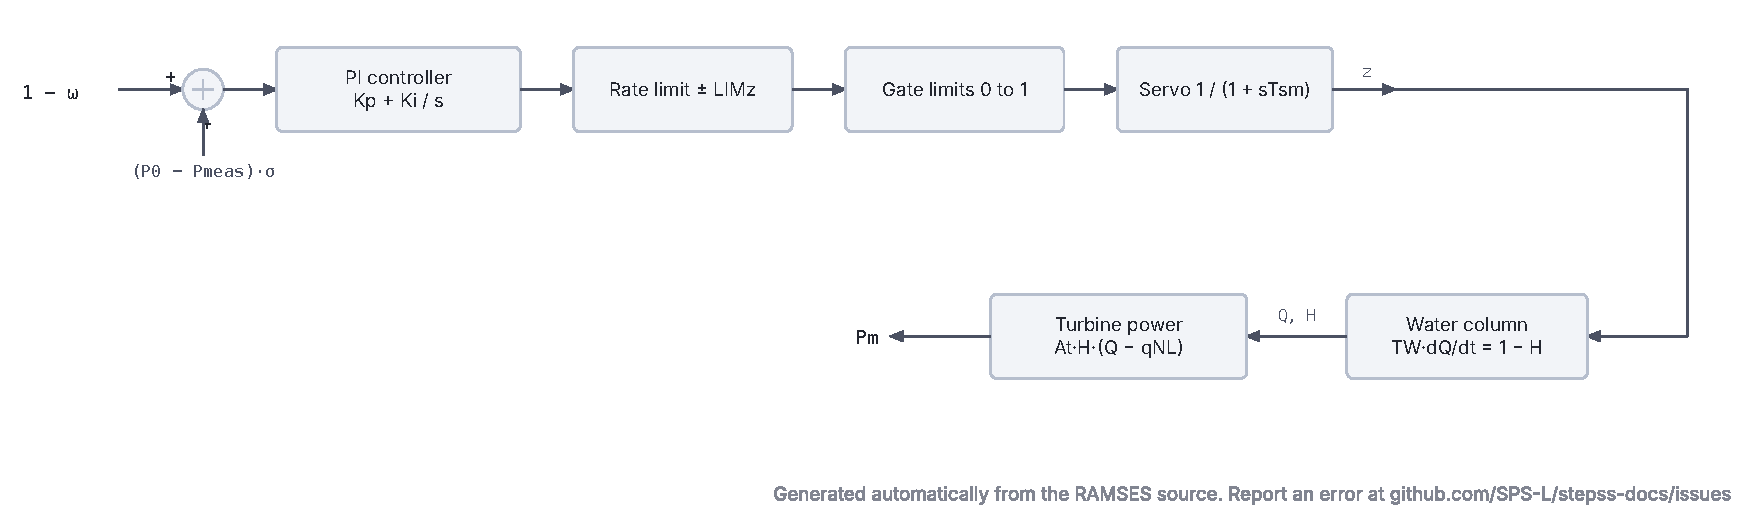
\includegraphics[width=0.98\linewidth]{figures/tor-hydro-generic1-light}
\caption{HYDRO\_GENERIC1 block diagram.}
\end{figure}

\subsection{Usage Example}\label{model-tor-generic:usage-example-3}

\textbf{RAMSES Data File}

\begin{Verbatim}
SYNC_MACH  g1  g1
      # FP FQ P Q: share of the power-flow injection (FP, FQ) or initial power (P in MW, Q in Mvar)
      1.  1.  0.  0.
      # SNOM: Nominal apparent power, used as base power in the machine model (MVA)
      800.
      # Pnom: Nominal active power of the turbine, used as base power for the turbine model (MW)
      760.
      # H: Inertia constant (s)
      3.
      # D: Damping coefficient (usually set to zero when the damper windings are modelled) (pu)
      0.
      # IBRATIO: Field current base ratio I_fB^mac/I_fB^exc (see above) (pu)
      0.95
      # TYPE_MOD: Parameter format keyword: RL or XT (case-insensitive)
      XT
      # Xl: Leakage reactance L_l (pu)
      0.15
      # Xd: d-axis synchronous reactance (pu)
      1.1
      # X'd: d-axis transient reactance (must be smaller than Xd) (pu)
      0.25
      # X"d: d-axis subtransient reactance (pu)
      0.2
      # Xq: q-axis synchronous reactance (pu)
      0.7
      # X'q: q-axis transient reactance (pu)
      *
      # X"q: q-axis subtransient reactance (pu)
      0.2
      # m: Saturation coefficient (set to 0 to neglect saturation)
      0.1
      # n: Saturation exponent (ignored when m = 0)
      6.0257
      # Ra: Armature resistance (pu)
      0.
      # T'do: d-axis open-circuit transient time constant (s)
      5.00
      # T"do: d-axis open-circuit subtransient time constant (s)
      0.05
      # T'qo: q-axis open-circuit transient time constant (s)
      *
      # T"qo: q-axis open-circuit subtransient time constant (s)
      0.1
EXC  GENERIC1
      # IFLIM: OEL field current threshold (pu)
      1.8991
      # d: OEL timer band, usually negative: timer runs down at rate 1 below IFLIM+d, holds between IFLIM+d and IFLIM (pu)
      -0.1
      # f: OEL timer charging rate offset above IFLIM
      0.
      # S: OEL timer charging rate per unit of field overcurrent (1/pu)
      1.
      # K1: Not used by the code
      100.
      # K2: OEL gain on (if - IFLIM), negative so that the OEL lowers excitation (pu/pu)
      -1.
      # L1: OEL timer lower limit and initial value, negative; the OEL acts when the timer exceeds 0 (s)
      -11
      # L2: OEL timer upper limit (s)
      10.
      # G: AVR gain (pu/pu)
      70.
      # TA: AVR lead time constant (s)
      10.
      # TB: AVR lag time constant (s)
      20.
      # TE: Exciter time constant (s)
      0.1
      # L3: Minimum field voltage (pu)
      0.
      # L4: Maximum field voltage (pu)
      4.
      # SPEEDIN: PSS input weight: 1 = speed, 0 = active power
      1
      # KPSS: PSS gain, derivative washout KPSS s/(1+sTw); 0 disables PSS (pu s)
      75.
      # Tw: PSS washout time constant (s)
      15.
      # T1: PSS first lead-lag numerator time constant (s)
      0.2
      # T2: PSS first lead-lag denominator time constant (s)
      0.01
      # T3: PSS second lead-lag numerator time constant (s)
      0.2
      # T4: PSS second lead-lag denominator time constant (s)
      0.01
      # DVMIN: PSS output lower limit (pu)
      -0.1
      # DVMAX: PSS output upper limit (pu)
      0.1
TOR  HYDRO_GENERIC1
      # SIGMA: permanent droop, gain on the power error P0 minus measured P (pu)
      0.04
      # Tmes: electrical power measurement time constant (s)
      2.0
      # Qv: no-load water flow (pu)
      0.
      # KP: PI proportional gain
      2.00
      # KI: PI integral gain (1/s)
      0.40
      # TSM: gate servomotor time constant (s)
      0.2
      # LIMZDOT: gate velocity limit, applied as plus or minus (pu/s)
      0.1
      # TW: water starting time (s)
      1.0
;
\end{Verbatim}

\textbf{Notes}

\begin{itemize}
\tightlist
\item
  \texttt{TW} (water-starting time) is the most influential parameter; typical values are 0.5--3 s.
\item
  Increase \texttt{KP} / \texttt{KI} carefully: large values can cause governor instability with high \texttt{TW}.
\item
  \texttt{Qv\ =\ 0} assumes no no-load losses.
\item
  Parameters follow the order in \texttt{dyn\_A.txt}: \texttt{SIGMA\ TP\ Qv\ KP\ KI\ TSM\ LIMZDOT\ TW}.
\end{itemize}

\begin{center}\rule{0.5\linewidth}{0.5pt}\end{center}

\section{\texorpdfstring{HYDRO\_DG (\texttt{tor\_HYDRO\_DG})}{HYDRO\_DG (tor\_HYDRO\_DG)}}\label{model-tor-generic:hydro_dg-tor_hydro_dg}

The data-file model name is \texttt{HYDRO\_DG}. Registered since 3.76.

\subsection{Scientific Description}\label{model-tor-generic:scientific-description-4}

A hydraulic turbine governor for a \textbf{dispersed generation unit that holds an active-power
setpoint and does not provide primary frequency response}.

The penstock and turbine are exactly those of \hyperref[model-tor-generic:hydro_generic1-tor_hydro_generic1]{\texttt{HYDRO\_GENERIC1}}.
What differs is the governor control law, and the difference is the point of the model.
\texttt{HYDRO\_GENERIC1} is a \textbf{speed governor}: its error signal carries an unconditional frequency
term, so the unit responds to system frequency whether or not that is wanted. \texttt{HYDRO\_DG}
regulates power alone.

\textbf{PI power regulator:}

The error is the deviation from the setpoint captured at initialisation, with no droop term
and no speed term:

\[e = P^{*} - P\]

\[\dot{x}_{I} = K_i \cdot e, \qquad z_{demand} = K_p \cdot e + x_{I}\]

There is no measurement lag on \(P\), so the regulator acts on the instantaneous electrical
power. The gate follows through a servo of time constant \(T_{sm}\), rate-limited to
\(\pm LIM_{\dot{z}}\) and position-limited to \([0, 1]\).

\textbf{Water column and turbine}, identical to \texttt{HYDRO\_GENERIC1}:

\[T_W \cdot \frac{dQ}{dt} = 1 - H, \qquad H = \left(\frac{Q}{z}\right)^{2}\]

\[T_m \cdot \omega = \frac{(Q - Q_v) \, H}{1 - Q_v}\]

\textbf{Parameters:}

\begin{small}\begin{longtable}[]{@{}lll@{}}
\toprule\noalign{}
Parameter & Index & Description \\
\midrule\noalign{}
\endhead
\bottomrule\noalign{}
\endlastfoot
\texttt{Qv} & 1 & No-load water flow fraction (pu) \\
\texttt{Kp} & 2 & PI proportional gain \\
\texttt{Ki} & 3 & PI integral gain \\
\texttt{TSM} & 4 & Gate servo time constant (s) \\
\texttt{LIMZDOT} & 5 & Gate velocity limit (pu/s) \\
\texttt{TW} & 6 & Water starting time (s) \\
\end{longtable}\end{small}

These are exactly parameters 3 to 8 of \texttt{HYDRO\_GENERIC1}, in the same order. \texttt{HYDRO\_GENERIC1}
precedes them with \texttt{SIGMA} (droop) and \texttt{Tmes} (speed measurement lag), and those two are what
\texttt{HYDRO\_DG} does not have. Setting \texttt{SIGMA} to zero in \texttt{HYDRO\_GENERIC1} does \textbf{not} reproduce
\texttt{HYDRO\_DG}, because the frequency term survives.

\textbf{Implementation details:}
- \texttt{nbxvar\ =\ 5}, \texttt{nbzvar\ =\ 2}, \texttt{nbdata\ =\ 6}, \texttt{nbaddpar\ =\ 1}
- Additional: \texttt{prm(7)\ =\ Pset}, the initial electrical power, captured at initialisation
- Observables: \texttt{z}, \texttt{Q}, \texttt{H}, \texttt{Pm}, \texttt{Pset}

\begin{figure}[htbp]
\centering
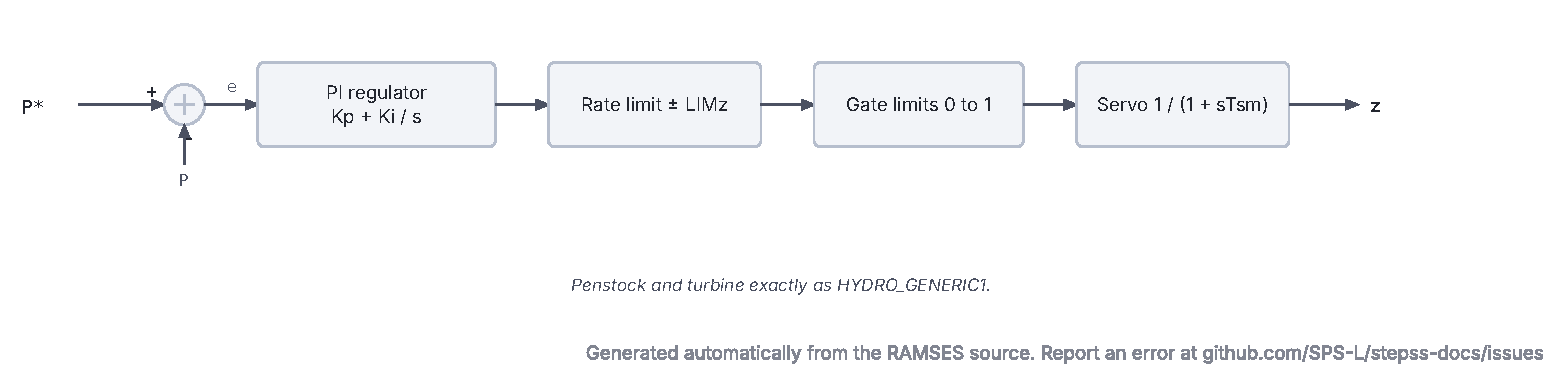
\includegraphics[width=0.98\linewidth]{figures/tor-hydro-dg-light}
\caption{HYDRO\_DG block diagram.}
\end{figure}

\subsection{Usage Example}\label{model-tor-generic:usage-example-4}

\textbf{RAMSES Data File}

\begin{Verbatim}
SYNC_MACH  G4  N4
      # FP FQ P Q: share of the power-flow injection (FP, FQ) or initial power (P in MW, Q in Mvar)
      1.  1.  0.  0.
      # SNOM: Nominal apparent power, used as base power in the machine model (MVA)
      5
      # Pnom: Nominal active power of the turbine, used as base power for the turbine model (MW)
      4.5
      # H: Inertia constant (s)
      3.
      # D: Damping coefficient (usually set to zero when the damper windings are modelled) (pu)
      0.
      # IBRATIO: Field current base ratio I_fB^mac/I_fB^exc (see above) (pu)
      1.9333
      # TYPE_MOD: Parameter format keyword: RL or XT (case-insensitive)
      XT
      # Xl: Leakage reactance L_l (pu)
      0.0937
      # Xd: d-axis synchronous reactance (pu)
      2.027
      # X'd: d-axis transient reactance (must be smaller than Xd) (pu)
      0.210
      # X"d: d-axis subtransient reactance (pu)
      0.173
      # Xq: q-axis synchronous reactance (pu)
      2.027
      # X'q: q-axis transient reactance (pu)
      *
      # X"q: q-axis subtransient reactance (pu)
      0.173
      # m: Saturation coefficient (set to 0 to neglect saturation)
      0.1
      # n: Saturation exponent (ignored when m = 0)
      6
      # Ra: Armature resistance (pu)
      0.00
      # T'do: d-axis open-circuit transient time constant (s)
      3.1
      # T"do: d-axis open-circuit subtransient time constant (s)
      0.0387
      # T'qo: q-axis open-circuit transient time constant (s)
      *
      # T"qo: q-axis open-circuit subtransient time constant (s)
      0.0387
EXC  AVR_DG
      # IFLIM: OEL field current threshold (pu)
      2.865
      # d: OEL timer band, usually negative: timer runs down at rate 1 below IFLIM+d, holds between IFLIM+d and IFLIM (pu)
      -0.1
      # f: OEL timer charging rate offset above IFLIM
      0.
      # S: OEL timer charging rate per unit of field overcurrent (1/pu)
      1.
      # K1: Not used by the code
      100.
      # K2: OEL gain on field current error if minus IFLIM (pu/pu)
      -1.
      # L1: OEL timer lower limit (initial value) (s)
      -20
      # L2: OEL timer upper limit (s)
      10
      # G: AVR gain (pu/pu)
      50
      # TA: AVR lead time constant (s)
      4
      # TB: AVR lag time constant (s)
      20
      # TE: Exciter time constant (s)
      0.1
      # L3: Minimum field voltage (pu)
      0
      # L4: Maximum field voltage (pu)
      5
      # SPEEDIN: PSS input weight: 1 = speed, 0 = active power
      1
      # KPSS: PSS gain, derivative washout KPSS s/(1+sTw); 0 disables PSS (pu s)
      0.
      # Tw: PSS washout time constant (s)
      5.
      # T1: PSS first lead-lag numerator time constant (s)
      1.
      # T2: PSS first lead-lag denominator time constant (s)
      1.
      # T3: PSS second lead-lag numerator time constant (s)
      1.
      # T4: PSS second lead-lag denominator time constant (s)
      1.
      # DVMIN: PSS output lower limit (pu)
      0.
      # DVMAX: PSS output upper limit (pu)
      0.
      # KQP: Reactive power regulator proportional gain (pu/pu)
      0.04
      # KQI: Reactive power regulator integral gain (1/s)
      0.06
      # L5: Reactive power regulator output lower limit (pu)
      -0.2
      # L6: Reactive power regulator output upper limit (pu)
      0.33
TOR  HYDRO_DG
      # Qv: no-load water flow (pu)
      0.0
      # Kp: PI proportional gain on power error
      0.1
      # Ki: PI integral gain on power error (1/s)
      0.4
      # TSM: gate servomotor time constant (s)
      0.2
      # LIMZDOT: gate velocity limit, applied as plus or minus (pu/s)
      0.1
      # TW: water starting time (s)
      1.0
;
\end{Verbatim}

\textbf{Notes}

\begin{itemize}
\tightlist
\item
  The setpoint is \textbf{not} a parameter. \texttt{Pset} is captured from the power-flow solution at
  initialisation, so the unit holds whatever it was dispatched to.
\item
  Because there is no frequency term, a system built only of these units has no primary
  frequency control. That is deliberate for dispersed generation studies, and it is worth
  being explicit about when interpreting a frequency response.
\item
  \texttt{Qv\ =\ 0} assumes no no-load losses.
\item
  The head relation divides by the gate position, which is floored at 1e-3 in the
  implementation so a fully closed gate cannot produce a division by zero.
\end{itemize}
